%%%%%%%%%%%%%%%%%%%%%%%%%%%%%%%%%%%%%%%%%%%%%%%%%%%%%
%                                                   %
%     Penn State Colloquium Poster Template         %
%                                                   %
% Uses Penn State Colloquium class, with options:   %
%                                                   %
% Orientation:                                      %
%     portrait (default), landscape                 %
%                                                   %
% Paper size:                                       %
%     a4paper (default), a0paper, a1paper, a2paper, %
%     a3paper, a5paper, a6paper                     %
%%%%%%%%%%%%%%%%%%%%%%%%%%%%%%%%%%%%%%%%%%%%%%%%%%%%%
\documentclass{../psuposter}
\renewcommand{\templateimagepath}{../} 


%%%%%%%%%%%%%%%%%%%%%%%%%%%%%%%%%%%%%%%%%%%%%%%%%%%%%
%               Package Dependencies                %
%%%%%%%%%%%%%%%%%%%%%%%%%%%%%%%%%%%%%%%%%%%%%%%%%%%%%
\usepackage{natbib}
\usepackage{lipsum}                                % Dummy text
\usepackage[figwidth = 0.98\linewidth]{todonotes}  % Dummy image (and more!)
\usepackage[absolute, overlay]{textpos}            % Figure placement
\usepackage{braket}
\setlength{\TPHorizModule}{\paperwidth}
\setlength{\TPVertModule}{\paperheight}
\setcitestyle{numbers,square}


%%%%%%%%%%%%%%%%%%%%%%%%%%%%%%%%%%%%%%%%%%%%%%%%%%%%%
%                 AUTHOR AND TITLE                  %
%%%%%%%%%%%%%%%%%%%%%%%%%%%%%%%%%%%%%%%%%%%%%%%%%%%%%
\title{Element synthesis and neutrinos in neutron star mergers}
\author{Gail McLaughlin}
\institute{North Carolina State University}


%%%%%%%%%%%%%%%%%%%%%%%%%%%%%%%%%%%%%%%%%%%%%%%%%%%%%
%                  BEGIN DOCUMENT                   %
%%%%%%%%%%%%%%%%%%%%%%%%%%%%%%%%%%%%%%%%%%%%%%%%%%%%%
\begin{document}
\begin{frame}
\begin{columns}[t, totalwidth=\textwidth]
\begin{column}{0.45\textwidth - 1cm}


%%%%%%%%%%%%%%%%%%%%%%%%%%%%%%%%%%%%%%%%%%%%%%%%%%%%%
%                 BLOCK: BIOGRAPHY                  %
%%%%%%%%%%%%%%%%%%%%%%%%%%%%%%%%%%%%%%%%%%%%%%%%%%%%%
    \begin{block}{Speaker Biographic Summary}
    	\begin{center}
    		
\includegraphics[width=0.68\textwidth]{images/portrait}
    	\end{center}
    	\href{https://physics.sciences.ncsu.edu/people/gcmclaug/}{Dr. Gail McLaughlin} is a Distinguished University Professor in Physics at North Carolina State University. She received her PhD in 1996 from the University of California San Diego. She was a postdoctoral research associate first at the Institute for Nuclear Theory at the University of Washington from 1996-1998, and then at TRIUMF from 1998-2000. From 2000-2001, she was a research scientist at the State University of New York, Stony Brook. She joined NC State University in 2001 as an Assistant Professor, and became an Associate Professor in 2005. She received an Outstanding Junior faculty Award from the Department of Energy, 2002-2007, and was also offered an NSF CAREER award in 2002. She has served on a number of committees which advise on policy nationally, such as the Nuclear Physics committee for Implementation the Long Range Plan, and the executive committee of the APS Division of Nuclear Physics. She is a member of the editorial board for Journal of Physics G.
    \end{block}


%%%%%%%%%%%%%%%%%%%%%%%%%%%%%%%%%%%%%%%%%%%%%%%%%%%%%
%            BLOCK: RESEARCH INTERESTS              %
%%%%%%%%%%%%%%%%%%%%%%%%%%%%%%%%%%%%%%%%%%%%%%%%%%%%%
    \begin{block}{Research Interests}
        Professor McLaughlin works in the areas of nuclear and particle astrophysics. This includes neutrinos in astrophysical environments, both their effect on the environment as well as the potential for detecting the neutrinos which make their way to earth. She is known for her work on neutrino interactions during the formation of the rapid neutron capture elements, theoretical studies of the detection of supernova neutrinos, and work on theories which create a neutrino magnetic moment.    
        \begin{center}
	    	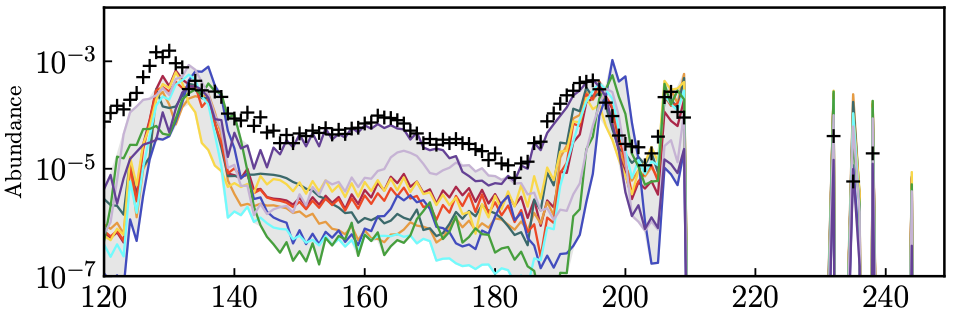
\includegraphics[width=0.8\textwidth]{images/research}   
	    	
	    	\textit{Abundance pattern different electron fractions. \cite{zhuModelingKilonovaLight2020}} 		
    	\end{center}
    	
    \end{block}
\end{column}
\begin{column}{0.55\textwidth - 1cm}


%%%%%%%%%%%%%%%%%%%%%%%%%%%%%%%%%%%%%%%%%%%%%%%%%%%%%
%                 BLOCK: ABSTRACT                   %
%%%%%%%%%%%%%%%%%%%%%%%%%%%%%%%%%%%%%%%%%%%%%%%%%%%%%
    \begin{block}{Talk Abstract}
    	The merging of two neutron stars is a true multimessenger event which includes gravitational waves, an electromagnetic signal and the emission of enormous numbers of neutrinos. In order to understand these signals we need a careful accounting of the microphysics that occurs during and after the merger. I will focus on the elements produced in these objects and the effect of two aspects of this microphysics; nuclear models/reactions and neutrino flavor transformation physics.  In particular, I will relate new developments in these areas to predictions of kilonova light curves and the astrophysical origin of the r-process.
    \end{block}


%%%%%%%%%%%%%%%%%%%%%%%%%%%%%%%%%%%%%%%%%%%%%%%%%%%%%
%                BLOCK: BACKGROUND                  %
%%%%%%%%%%%%%%%%%%%%%%%%%%%%%%%%%%%%%%%%%%%%%%%%%%%%%
    \begin{block}{Brief Background}
    	Thought to be one of the main mechanisms by which heavy, beyond-iron isotopes are synthesized, the \textit{r-process} entails a succession of neutron captures so rapid that the seed nuclei do not have time to undergo radioactive decay between captures. The astrophysical origins of the r-process are still being investigated; however, neutron star mergers (NSM) have been confirmed as one source of the r-process in the universe. Though the degree to which NSM account for r-process material remains unclear, recent work has connected NS merger outflow to stellar abundances and mass distributions using various equations of state (EOS). \cite{holmbeckReconstructingMassesMerging2020}\\
    	%\cite{longLocalAxonalConduction2020} 
        \begin{center}
		   	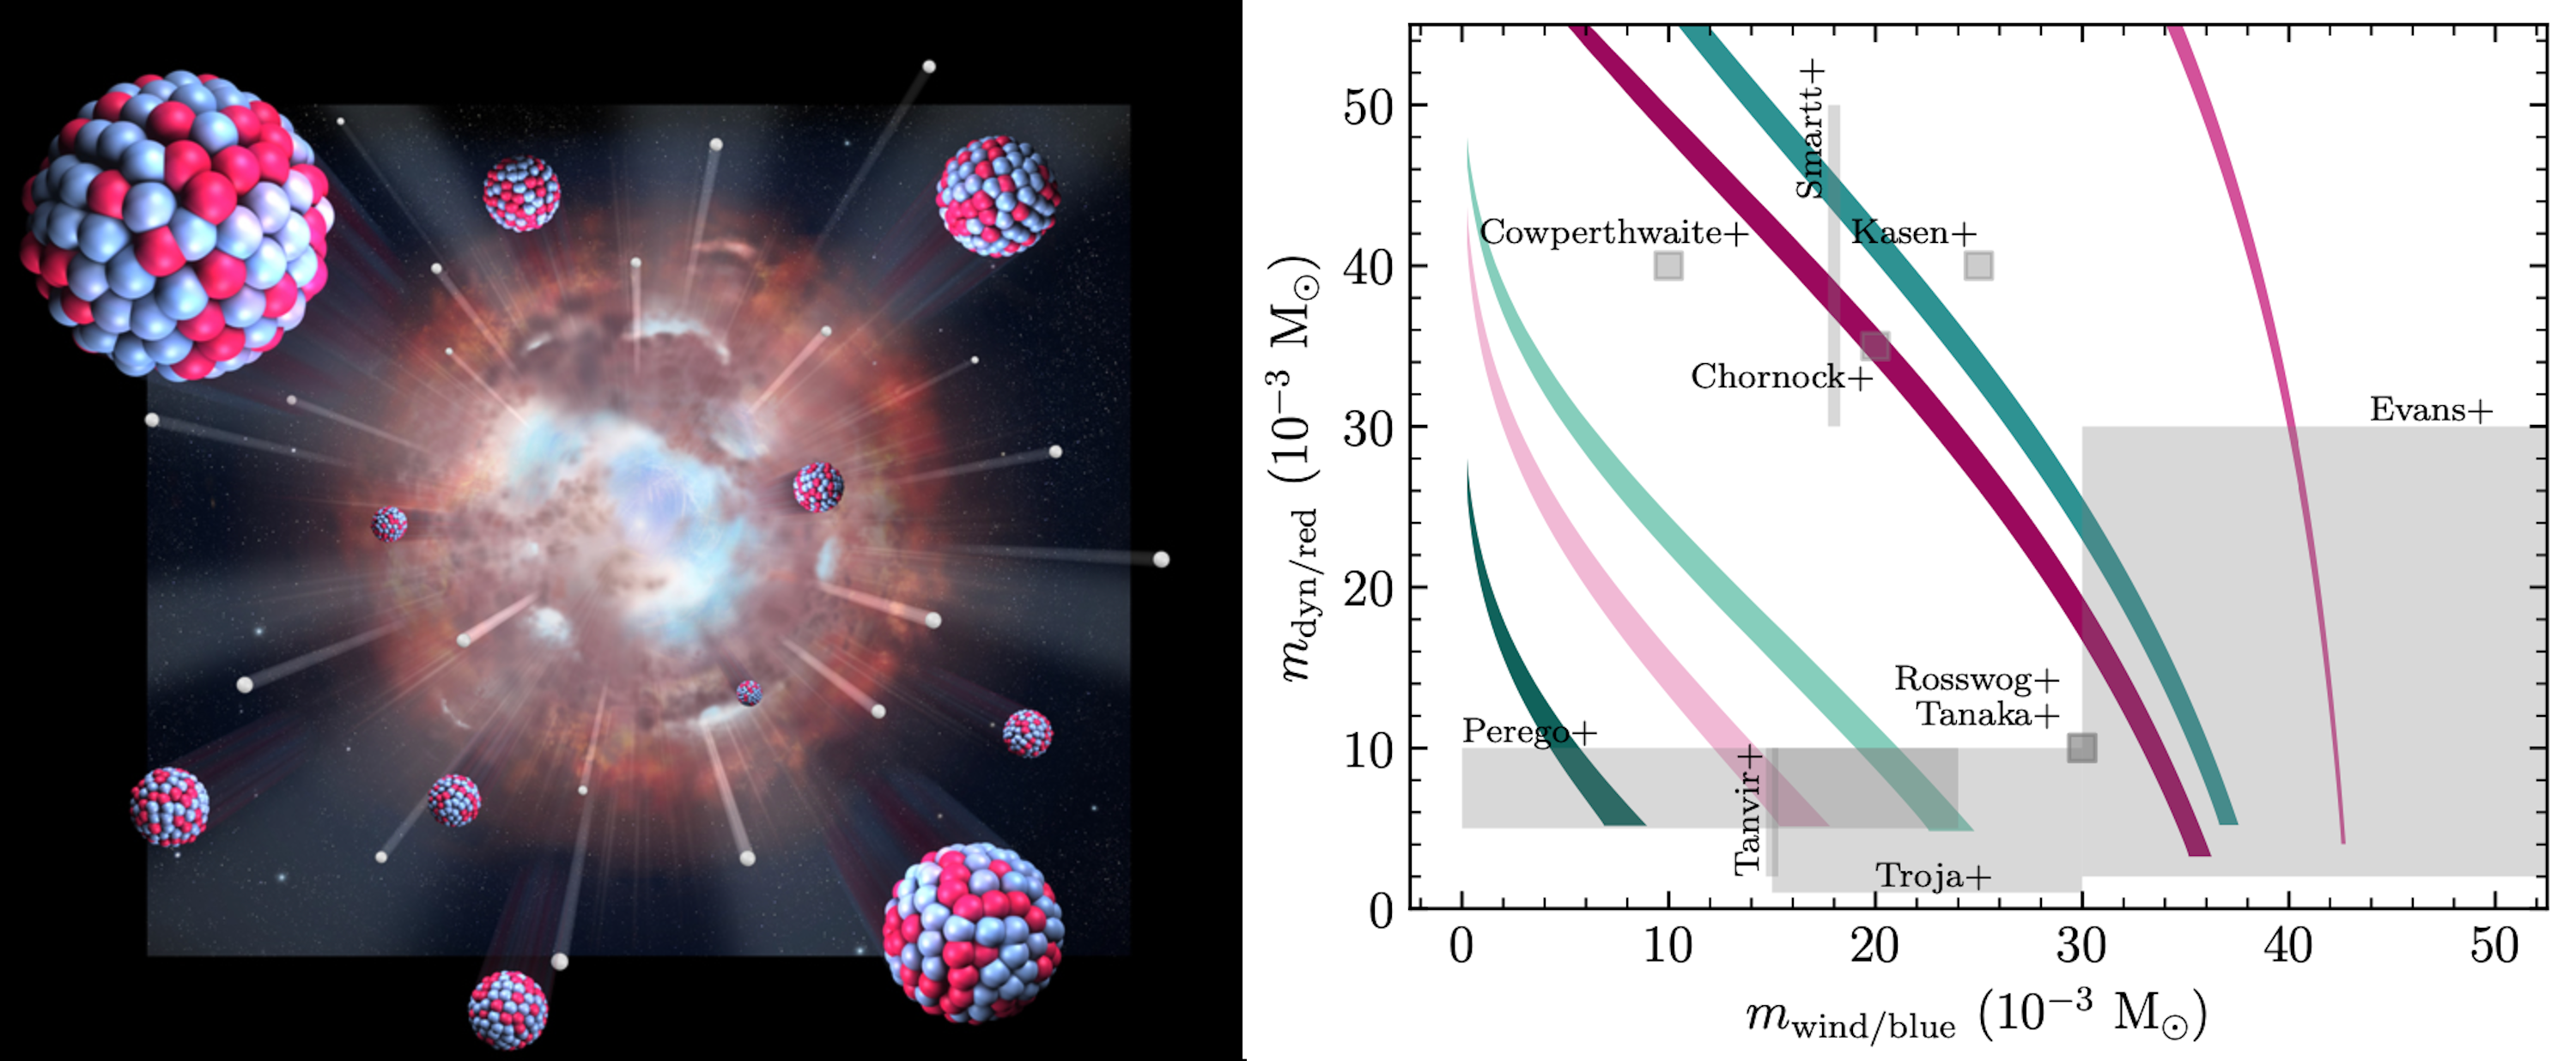
\includegraphics[width=0.95\textwidth]{images/background}    		
		   	\newline
		   	
		   	\textit{Left: Rendering of r-process producing heavy nuclei in a supernova. \cite{mikamiGreatProgressOrigin}
		   	Right: Predicted ejecta masses from GW170817 for various EOS. \cite{holmbeckReconstructingMassesMerging2020}}
    	\end{center} 
		%\cite{longMorphologicalCharacterizationHVC2018} 
    \end{block}


%%%%%%%%%%%%%%%%%%%%%%%%%%%%%%%%%%%%%%%%%%%%%%%%%%%%%
%                 BLOCK: REFERENCES                 %
%%%%%%%%%%%%%%%%%%%%%%%%%%%%%%%%%%%%%%%%%%%%%%%%%%%%%
\nocite{*}
    \begin{block}{References}

        \bibliographystyle{aipnum4-1}
%        \bibliographystyle{iopart-num}
		\bibliography{references}
    \end{block}

\end{column}
\end{columns}


%%%%%%%%%%%%%%%%%%%%%%%%%%%%%%%%%%%%%%%%%%%%%%%%%%%%%
%                    FOOTER TEXT                    %
%%%%%%%%%%%%%%%%%%%%%%%%%%%%%%%%%%%%%%%%%%%%%%%%%%%%%
\begin{textblock}{0.5}(0.18, 0.94)
    \color{white}
    \sffamily
    \textbf{Eberly College of Science}
    \\
    Department of Physics
\end{textblock}


%%%%%%%%%%%%%%%%%%%%%%%%%%%%%%%%%%%%%%%%%%%%%%%%%%%%%
%                   END TEMPLATE                    %
%%%%%%%%%%%%%%%%%%%%%%%%%%%%%%%%%%%%%%%%%%%%%%%%%%%%%
\end{frame}
\end{document}
